\documentclass[10pt, letter]{article}
\newcommand{\doctitle}{%
CS 7650 Natural Language Processing}
\newcommand{\bigO}{\ensuremath{\mathcal{O}}}
\usepackage{graphicx}
\usepackage{float}
\usepackage{listings}
\usepackage{comment}
\usepackage{fancyvrb}
\usepackage{booktabs}
\usepackage[usenames,dvipsnames]{color}
\usepackage[center]{caption}
\usepackage{algorithm}
\usepackage[T1]{fontenc}
\usepackage{algpseudocode}
\usepackage[margin=1in]{geometry}
\usepackage[usenames,dvipsnames]{color}
\usepackage{hyperref}
\hypersetup{
  colorlinks,
  citecolor=Violet,
  linkcolor=Black,
  urlcolor=Blue}
\begin{document}
\title{\textsc{Project \#3: Parsing} \\ \textbf{\doctitle}}
  \author {Arvind Krishnaa Jagannathan \\ GT ID: 902891874}
   \date{March 04, 2013}
\maketitle
\section{CFG Parsing for Twitter}
\subsection{Getting Started}
\subsubsection*{Deliverable 1}
The CFG I created has 9 non-terminals. They are: 
\begin{enumerate}
	\item \textbf{S}: Corresponds to a sentence (or a tweet in this case). A sentence can be constructed recursively. In the case of the simple CFG which gives only one parse per sentence, a sentence can be constructed by concatenating two sentences with a conjunction, or a conjunction followed by a sentence (in regular English this would be incorrect), or a re-tweet marker followed by a sentence. In addition, in order to remove ambiguities, I do not have the 
	\begin{verbatim}	
		S -> NP VP
	\end{verbatim}
	production. Instead I have a production
	\begin{verbatim}
		S -> PHR
		PHR -> NP | VP
	\end{verbatim}
	and there are productions leading from a NP (noun phrase) to VP (verb phrase).
	\item \textbf{RT}: Corresponds to the re-tweet marker - a sequence of tags corresponding to the words RT @user :. Usually this marker can be found only at the start of a sentence. 
	\item \textbf{PHR}: Corresponds to a phrase. A phrase can be either a noun phrase (NP) or verb phrase (VP).
	\item \textbf{NP}: A noun phrase. This could either begin with a proper noun (``\textasciicircum''), a common noun (``N''), a pronoun (``O''), a nominal (``S''), proper noun + verbal (``M''), a nominal + verbal (``L''). It could be constructed recursively either by combining a NP with a prepositional phrase (PP) or a verb phrase (VP), adjectival phrase (ADJP), adverbial phrase (ADVP) or a special character (Z).
	\item \textbf{VP}: A verb phrase. This could be constructed by a verb (``V'') followed by a particle (``T'') or an existential there (''X''). The verb phrase can be recursively constructed by combining one of these terminals with itself, or with a noun phrase, a prepositional phrase, an adverbial phrase, adjectival phrase or special character.
	\item \textbf{ADJP}: An adjectival phrase. It is a non-terminal preceeded by one or more adjectives (``A'') and can also be constructed recursively from another ADJP.
	\item \textbf{ADVP}: An adverbial phrase. It is a non-terminal preceeded by one or more adverbs (``R''). This can also be recursively constructed from another ADVp.
	\item \textbf{PP}: A prepositional phrase. It is a non-terminal preceeded by one or more prepositions (``P'') or followed by a noun phrase or a verb phrase.
	\item \textbf{Z}: This non-terminal collects all the special characters/punctuations and numerals. One or more of these could compose Z.
\end{enumerate}
The CFG is called \textit{``jagannathan-task1.cfg"}. It is reproduced here,
\begin{verbatim}
S -> S "&" S | "&" S | RT S | PHR

RT -> "~" "@" "~"

PHR -> NP | VP

NP -> "^" | "N" | "O" | "S" | "M" | "Y" | "L" | Z
NP -> "^" VP | "N" VP | "O" VP | "S" VP | "M" VP | "Y" VP | "L" VP
NP -> "D" "N" "P"
NP -> "D" NP | "^" NP | "N" NP | "O" NP | "O" ADJP | Z NP | "S" NP | "L" NP | "M" NP
NP -> "Y" NP | "L" NP
NP -> "^" ADJP | "N" ADJP | "D" ADJP | "S" ADJP
NP -> "R" ADJP | "A" ADVP | "A" NP | "R" NP | "R" ADVP | "P" NP | "P" "V" NP

VP -> "V" | "V" "T"
VP -> "V" NP | "V" "T" NP
VP -> "V" ADVP | "V" ADJP
VP -> "V" NP | "V" VP | Z VP | "V" "T" VP
VP -> "A" VP | "R" VP | "X" VP

ADJP -> "A" | "A" ADJP

PP -> "P"
PP -> "P" NP | "P" VP

ADVP -> "R" | "R" ADVP

Z -> "," | "!" | "#" | "$" | "E" | "U" | "G" | "@"
\end{verbatim}
I got the following measures for this grammar. Notably. I get a F-measure of 35.97\%.
\begin{itemize}
	\item \textbf{Recall}: 1.0
	\item \textbf{Parses-per-sentence}: 1.0
	\item \textbf{F-Measure}: 0.3597359735973597
	\item \textbf{Precision}: 0.2193158953722334
\end{itemize}

\subsection{Grammar design}
\subsubsection*{Deliverable 2}
I have two grammars, \textit{``jagannathan-task2.cfg''} and \textit{``jagannathan-task2\_1.cfg''} which give perfect recall for the development data. Their F-Measures are 40.74\% and 41.52\% respectively, while the number of parses per sentence are 2.137 and 1.348 respectively. I have summarized the two grammars in Table \ref{table1}.

\begin{table}[htbp]
\centering
\begin{tabular}{|l|r|r|r|r|}
\hline
Context Free Grammar & \multicolumn{1}{l|}{Recall} & \multicolumn{1}{l|}{Parses per sentence} & \multicolumn{1}{l|}{F-Measure} & \multicolumn{1}{l|}{Precision} \\ \hline
\textit{jagannathan-task2.cfg} & 100.00\% & 2.137 & 40.74\% & 25.58\% \\ \hline
\textit{jagannathan-task2\_1.cfg} & 100.00\% & 1.348 & 41.52\% & 26.20\% \\ \hline
\end{tabular}
\caption{Two grammars for Deliverable 2}
\label{table1}
\end{table}

\subsubsection*{Deliverable 3}
Even after I change the \textbf{max\_len} parameter in the \textit{evalParser()} method, my two grammars do not produce that many more parses per sentence. However, the grammars no longer produce perfect recall. The summary of two grammars is shown in Table \ref{table2}.

\begin{table}[htbp]
\centering
\begin{tabular}{|l|r|r|r|r|}
\hline
Context Free Grammar & \multicolumn{1}{l|}{Recall} & \multicolumn{1}{l|}{Parses per sentence} & \multicolumn{1}{l|}{F-Measure} & \multicolumn{1}{l|}{Precision} \\ \hline
\textit{jagannathan-task2.cfg} & 81.70\% & 4.71875 & 42.80\% & 29.00\% \\ \hline
\textit{jagannathan-task2\_1.cfg} & 82.12\% & 2.507 & 45.35\% & 31.33\% \\ \hline
\end{tabular}
\caption{Comparison of two grammars when \textbf{max\_len} = 20}
\label{table2}
\end{table}

\subsubsection*{Deliverable 4}
In my grammar, I added the verbal tags as terminals which are at the head of a noun phrase. However, since these words (such as she'll) will usually be followed by a verb, so I have a production like
\begin{verbatim}
NP -> "L"
NP -> "L" VP
\end{verbatim}
and similarly for other verbal tags.

\subsection{Terminal Refinement}
\subsubsection*{Deliverable 5}
I made a few tag improvements based on the ideas in the paper on ``Accurate Unlexicalized Parsing'' by Klein and Manning \cite{klein2003accurate}. However, the F-Measure increased from 40.74\% (I used the first grammar \textit{``jagannathan-task2.cfg''}) to 42.91\% only. I present the summary of the new grammar in Table \ref{table3}.

\begin{table}[htbp]
\centering
\begin{tabular}{|l|r|r|r|r|}
\hline
Context Free Grammar & \multicolumn{1}{l|}{Recall} & \multicolumn{1}{l|}{Parses per sentence} & \multicolumn{1}{l|}{F-Measure} & \multicolumn{1}{l|}{Precision} \\ \hline
\textit{jagannathan-task3.cfg} & 94.49\% & 2.067 & 42.91\% & 27.54\% \\ \hline
\end{tabular}
\caption{Summary of new Grammar (compare with Table \ref{table1})}
\label{table3}
\end{table}

These are the changes which I made using the \textbf{preprocess()} function (in addition to assigning a special tag `2' for the word `to')
\begin{enumerate}
	\item If the special character is "." and is at the end of a sentence, then assign it a special tag. I did this so that I could have a production of the form,
	\begin{verbatim}
		S -> S "." S
	\end{verbatim}
	\item Whenever the word ``just'' is tagged as an adverb, I have changed the tag to `J'. This is as per \cite{klein2003accurate}. Then I have created a rule,
	\begin{verbatim}
		ADVP -> "J" ADVP
		NP -> "R" ADVP
	\end{verbatim}
	since the word ``just'' is mostly associated with noun phrases.
	\item The prepositions ``of'' and ``as'' are assigned their own tags. This is so that I could create new rules for a prepositional phrase, with ``of'' being associated with noun phrases and ``as'' with verb phrases.
	\begin{verbatim}
		PP -> "OF" NP | "AS" VP
	\end{verbatim}
\end{enumerate}
I was unable to think of many new modifications, because most of my original grammar was designed with the tagset from the Twitter POS tagging paper \cite{gimpel2010part} and my own knowledge of common tweet structures.

\subsubsection*{Deliverable 6}

My best grammars are \textit{``jagannathan1.cfg''} and \textit{``jagannathan2.cfg''}, which are the \textbf{same as that for deliverable 2}. Please note that these grammars gave me perfect recall for the development data and F-measure of 40.74\% and 41.52\% respectively. It would be great if both of these grammars (the second one has subtle development data specific production rules) could be evaluated on the test data.

\section{Unlabeled Dependency Parsing}
\subsubsection*{Deliverable 7}
When I run the \textit{read\_data()} the number of features I get are \textbf{801}.
\subsection{Training}
After 10 iterations of training, the dependency parser gives an accuracy of 50.97\%.
\subsection{More features}
\subsubsection*{Deliverable 8}
I obtain the distance from the head and the modifier and store it as,
\begin{verbatim}
head_modifier_distance = m - h
\end{verbatim}
As per the advice suggested, I set an upper threshold of 8 and a lower threshold of -5. That is,
\begin{verbatim}
if head_modifier_distance > 8:
   head_modifier_distance = 8
if head_modifier_distance < -5:
   head_modifier_distance = -5
\end{verbatim}
After adding the distance between the head and modifier as a feature, I get an accuracy of \textbf{64.07\%} and the number of features increased from 801 to \textbf{814}. The variation of accuracy with number of iterations on the development data, with no features, and after implementing the features of deliverable 8 are shown in Figure \ref{deli8}.
\begin{figure}[h!]
  \centering
    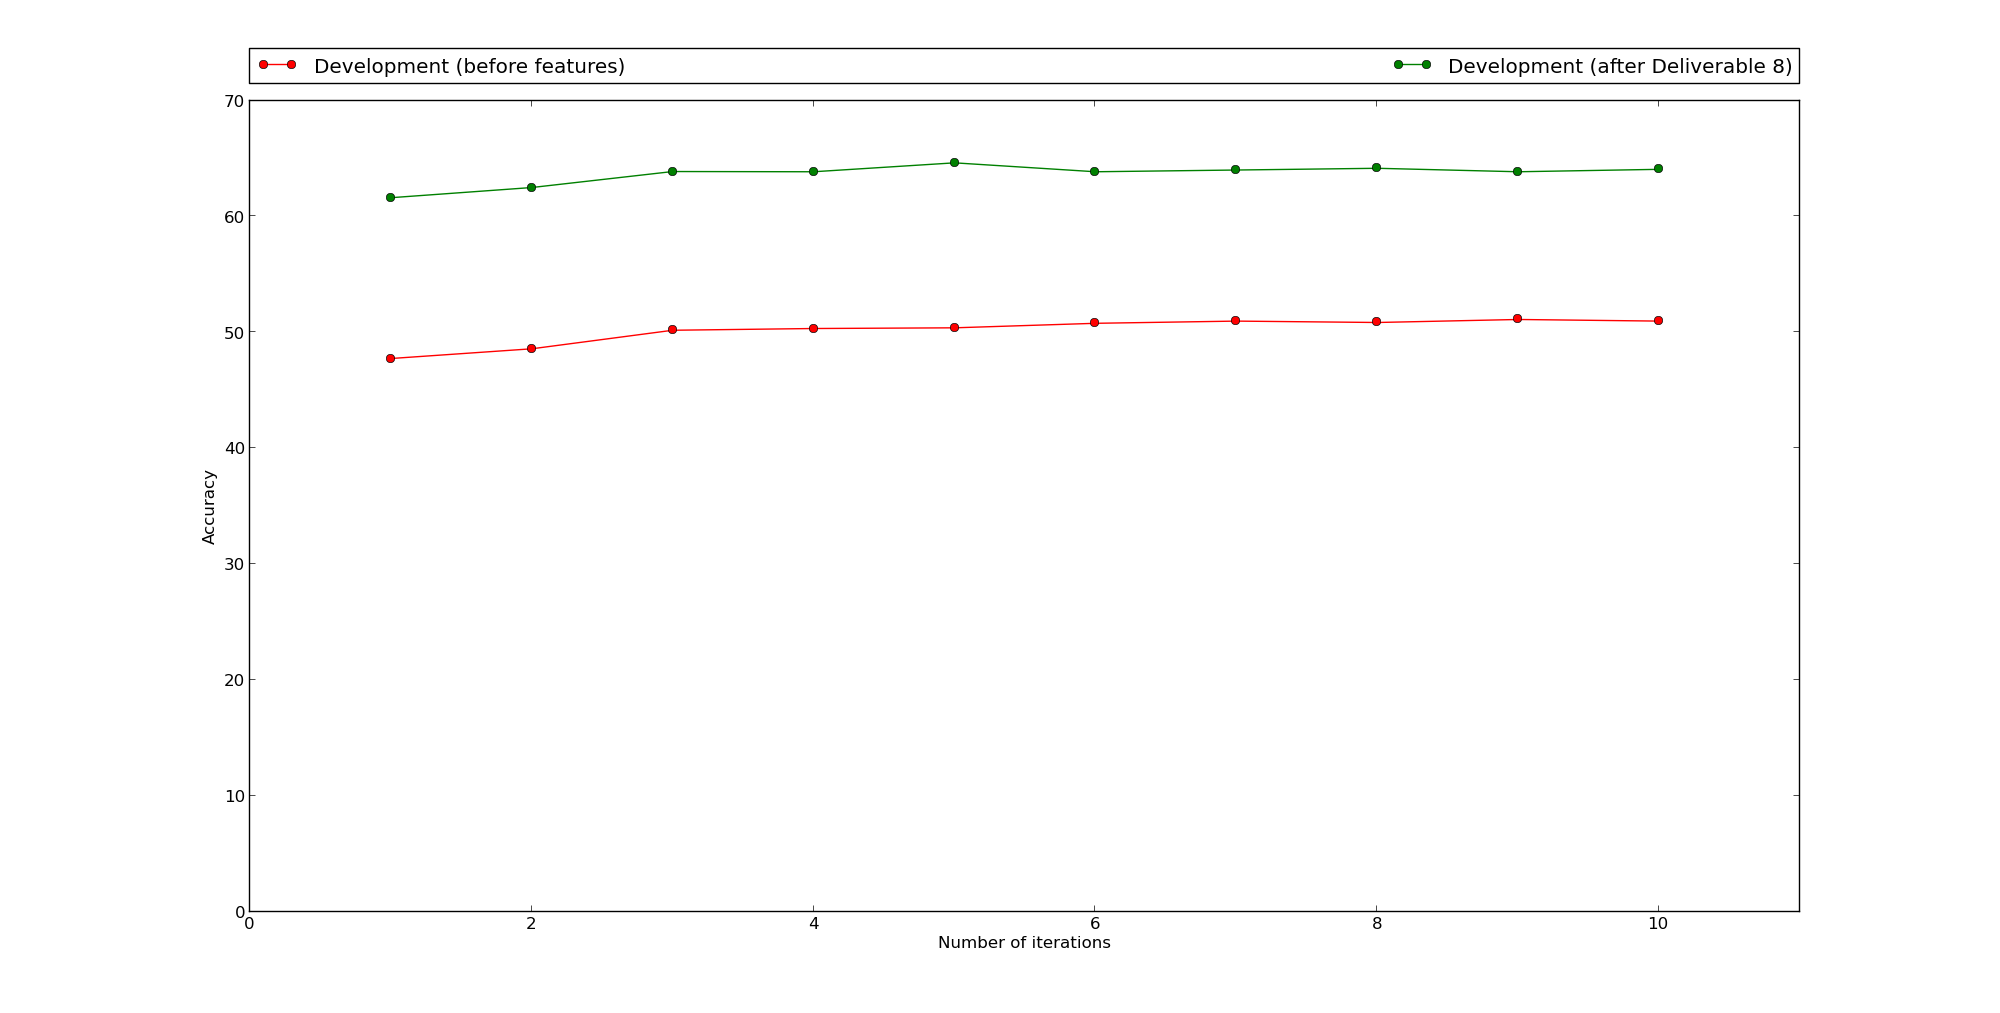
\includegraphics[scale = 0.25]{Images/deliverable8}
    \caption{Accuracy vs. Number of iterations for development with and without features}
  \label{deli8}
\end{figure}

\subsubsection*{Deliverable 9}
I added the two features - (a) lexical features between the word of the head and tag of the modifier (b) between the word of the modifier and tag of the head. This significantly pushed up the accuracy on the development data, to \textbf{75.23\%}. The accuracy on training data was \textbf{85.98\%} (both depicted in Figure \ref{deli9}). Also the number of features significantly went up to \textbf{44539}.

\begin{figure}[h!]
  \centering
    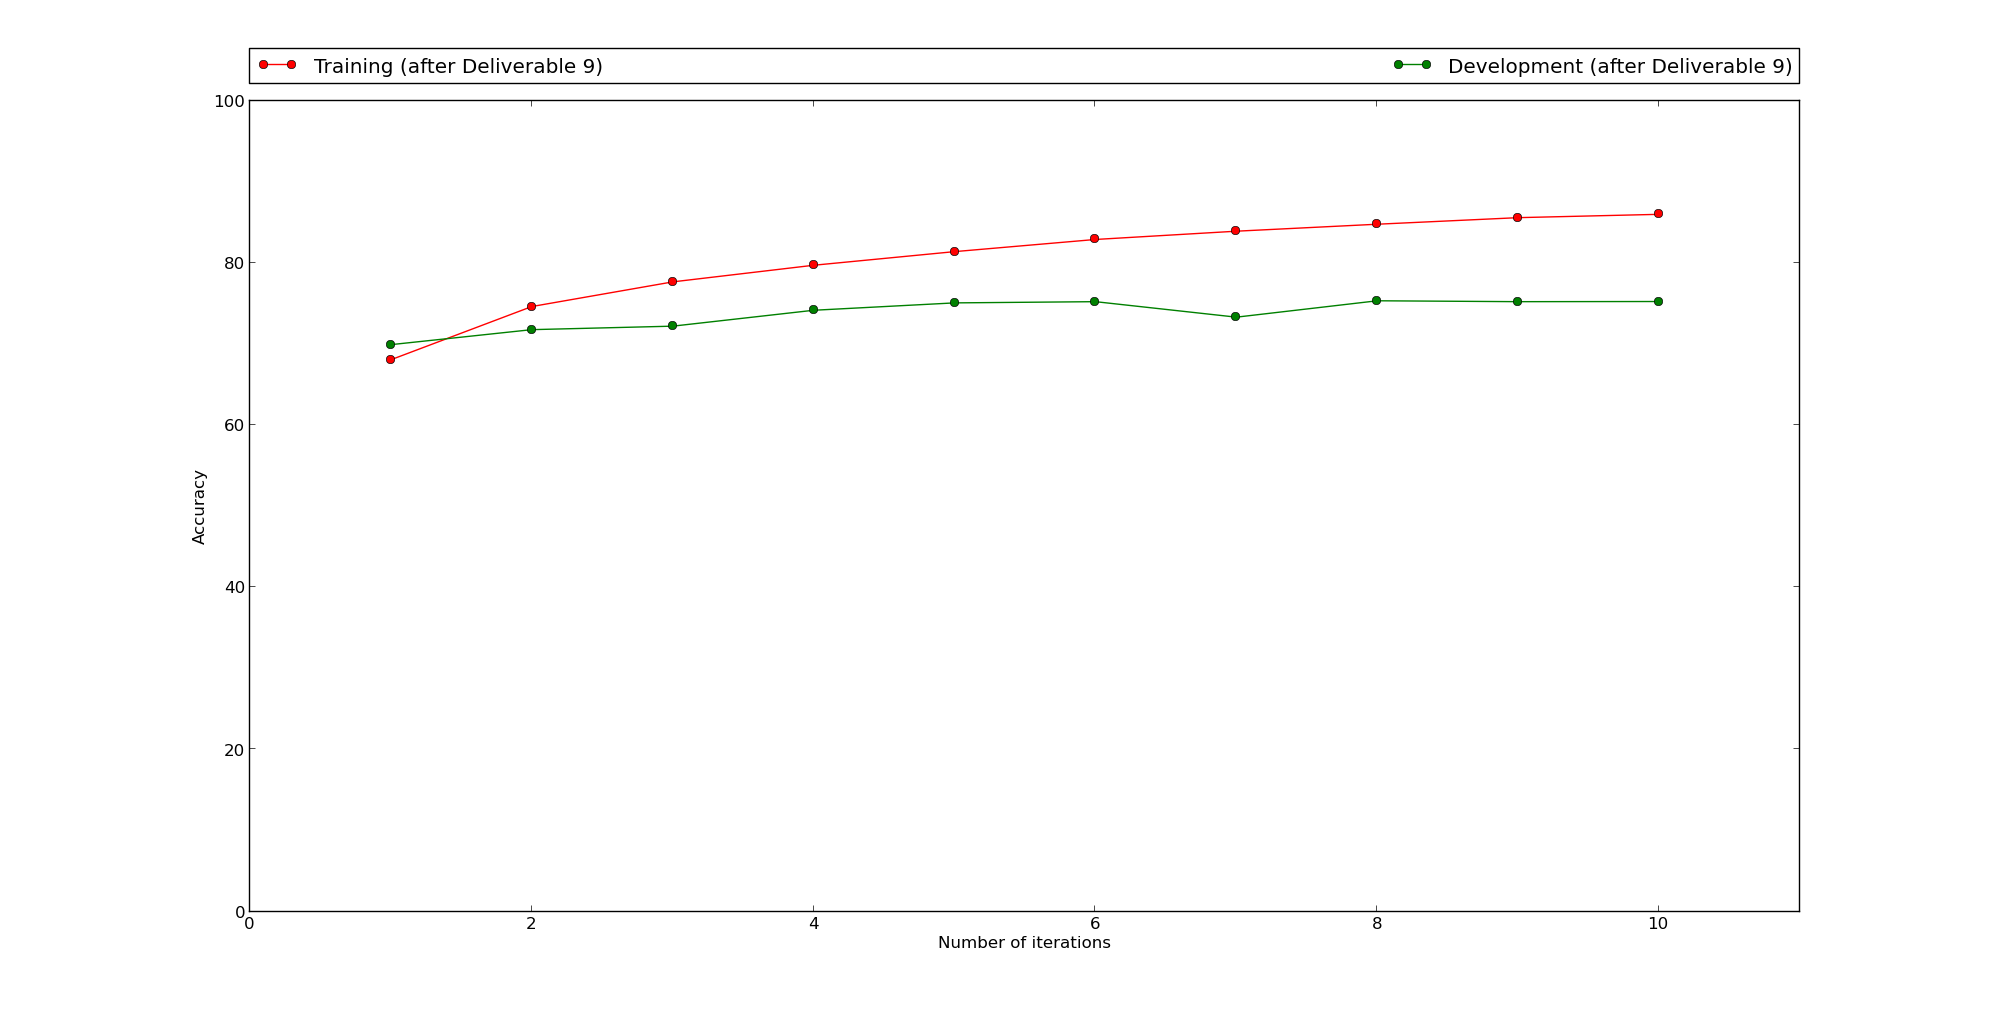
\includegraphics[scale = 0.25]{Images/deliverable9}
    \caption{Accuracy vs. Number of iterations for training and development data after Deliverable 9}
  \label{deli9}
\end{figure}

\subsubsection*{Deliverable 10}
After adding the bi-lexical features between the head and the modifier (i.e the word of the head and the word of the modifier), the number of features almost doubles to \textbf{88473}. Both the training and development data accuracy increased slightly to \textbf{92.29\%} and \textbf{76.78\%}. Figure \ref{deli10} represents this data.

\begin{figure}[h!]
  \centering
    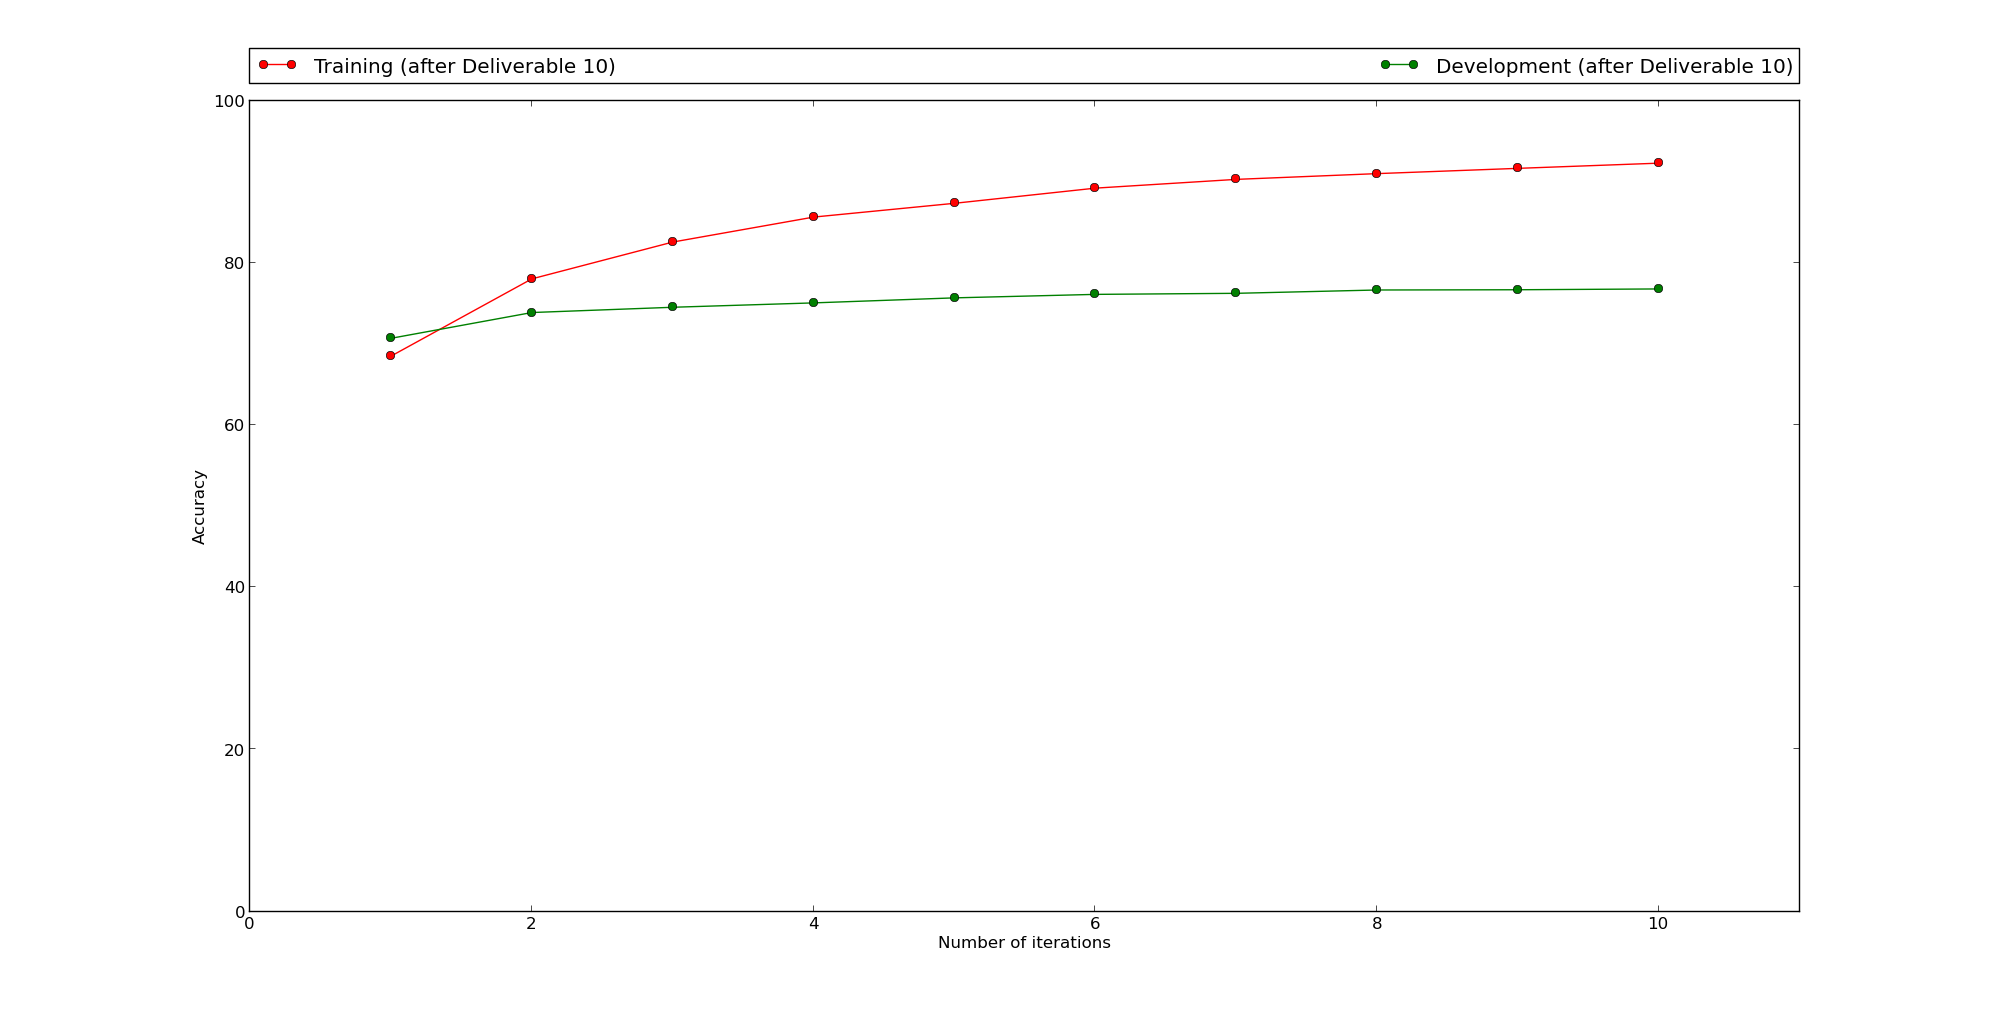
\includegraphics[scale = 0.25]{Images/deliverable10}
    \caption{Accuracy vs. Number of iterations for training and development data after Deliverable 10}
  \label{deli10}
\end{figure}

\subsubsection*{Deliverable 11}
I added the following context features (the ones mentioned in the assignment + a few more combinations):
\begin{itemize}
	\item $<t[h]; t[h - 1]; t[m]>$: head, head-left, modifier
	\item $<t[h]; t[m]; t[m + 1]>$: head, modifier, modifier-right
	\item $<t[h]; t[m - 1]; t[m]>$: head, modifier-left, modifier
	\item $<t[h]; t[h - 1]; t[m]; t[m + 1]>$: head, head-left, modifier, modifier-right
	\item $<t[h]; t[h - 1]; t[m]; t[m - 1]>$: head, head-left, modifier, modifier-left
	\item $<t[h]; t[h + 1]; t[m]; t[m - 1]>$: head, head-right, modifier, modifier-left
	\item $<t[h]; t[h + 1]; t[m]; t[m + 1]>$: head, head-right, modifier, modifier-right
	\item $<t[h]; t[h - 1]; t[h + 1]; t[m]; t[m + 1]>$: head, head-left, head-right, modifier, modifier-right
	\item $<t[h]; t[h - 1]; t[h + 1]; t[m]; t[m - 1]>$: head, head-left, head-right, modifier, modifier-left
	\item $<t[h]; t[h - 1]; t[h + 1]; t[m]; t[m - 1]; t[m + 1]>$: head, head-left, head-right, modifier-left, modifier, modifier-right
	\item $<t[h]; t[h + k] ; t[m]>$: for k in (1, head\_modifier\_distance). head, all head-rights, modifier
	\item $<t[h]; t[m - k] ; t[m]>$ for k in (1, head\_modifier\_distance). head, all modifier-lefts, modifier
\end{itemize}
\textbf{Note}: I got the idea for the last two features from the paper for literature review.

I tried a few more combinations too, but beyond a point, the number of features went too high, making the program slow, but did not improve the accuracy rate at all. With the above mentioned context features, the total number of features come up to \textbf{273415}. The accuracy of training data and development data go upto \textbf{98.53\%} and \textbf{89.39\%} respectively. Figure \ref{deli11} shows the how adding these features affects training and development accuracy.

\begin{figure}[h!]
  \centering
    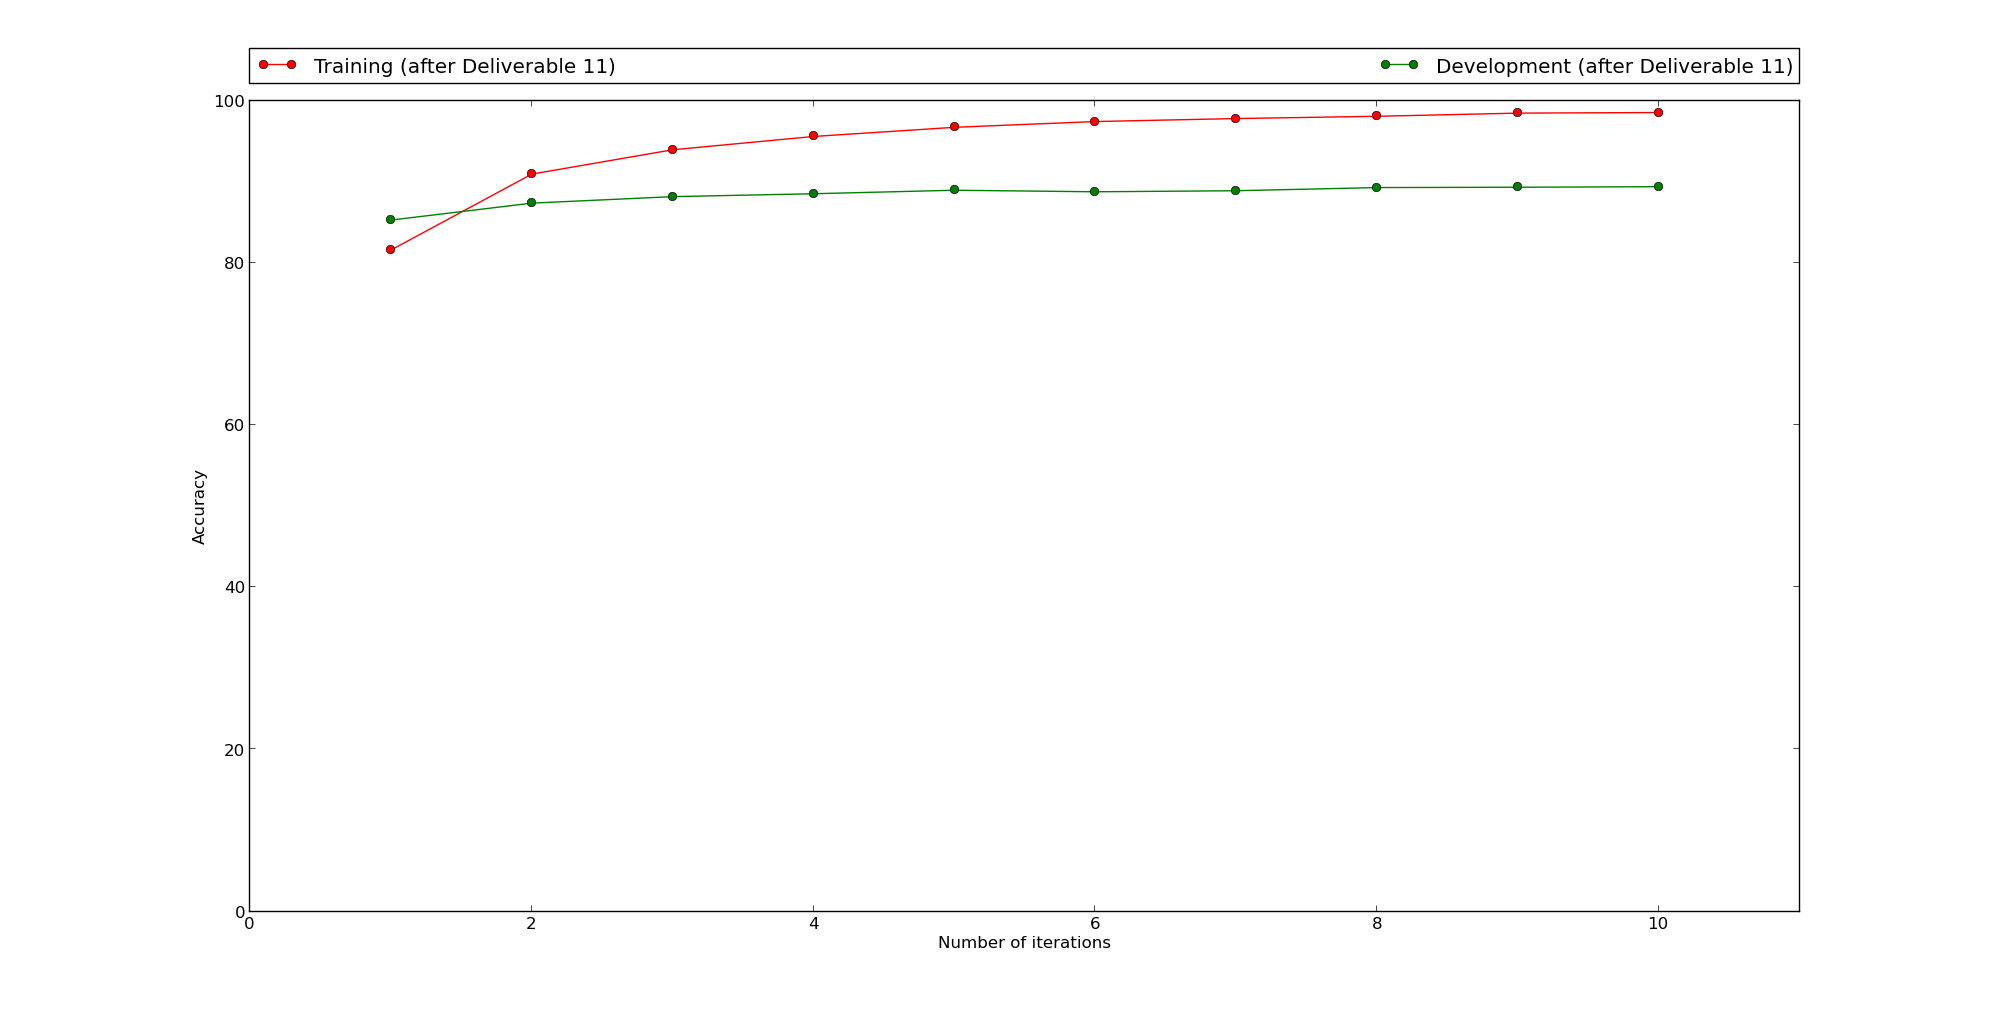
\includegraphics[scale = 0.25]{Images/deliverable11}
    \caption{Accuracy vs. Number of iterations for training and development data after Deliverable 11}
  \label{deli11}
\end{figure}

The increase in the number of features, from deliverable 7 (pair of tags in dependency arc) to deliverable 11 (context features) is depicted in Figure \ref{fig}

\begin{figure}[h!]
  \centering
    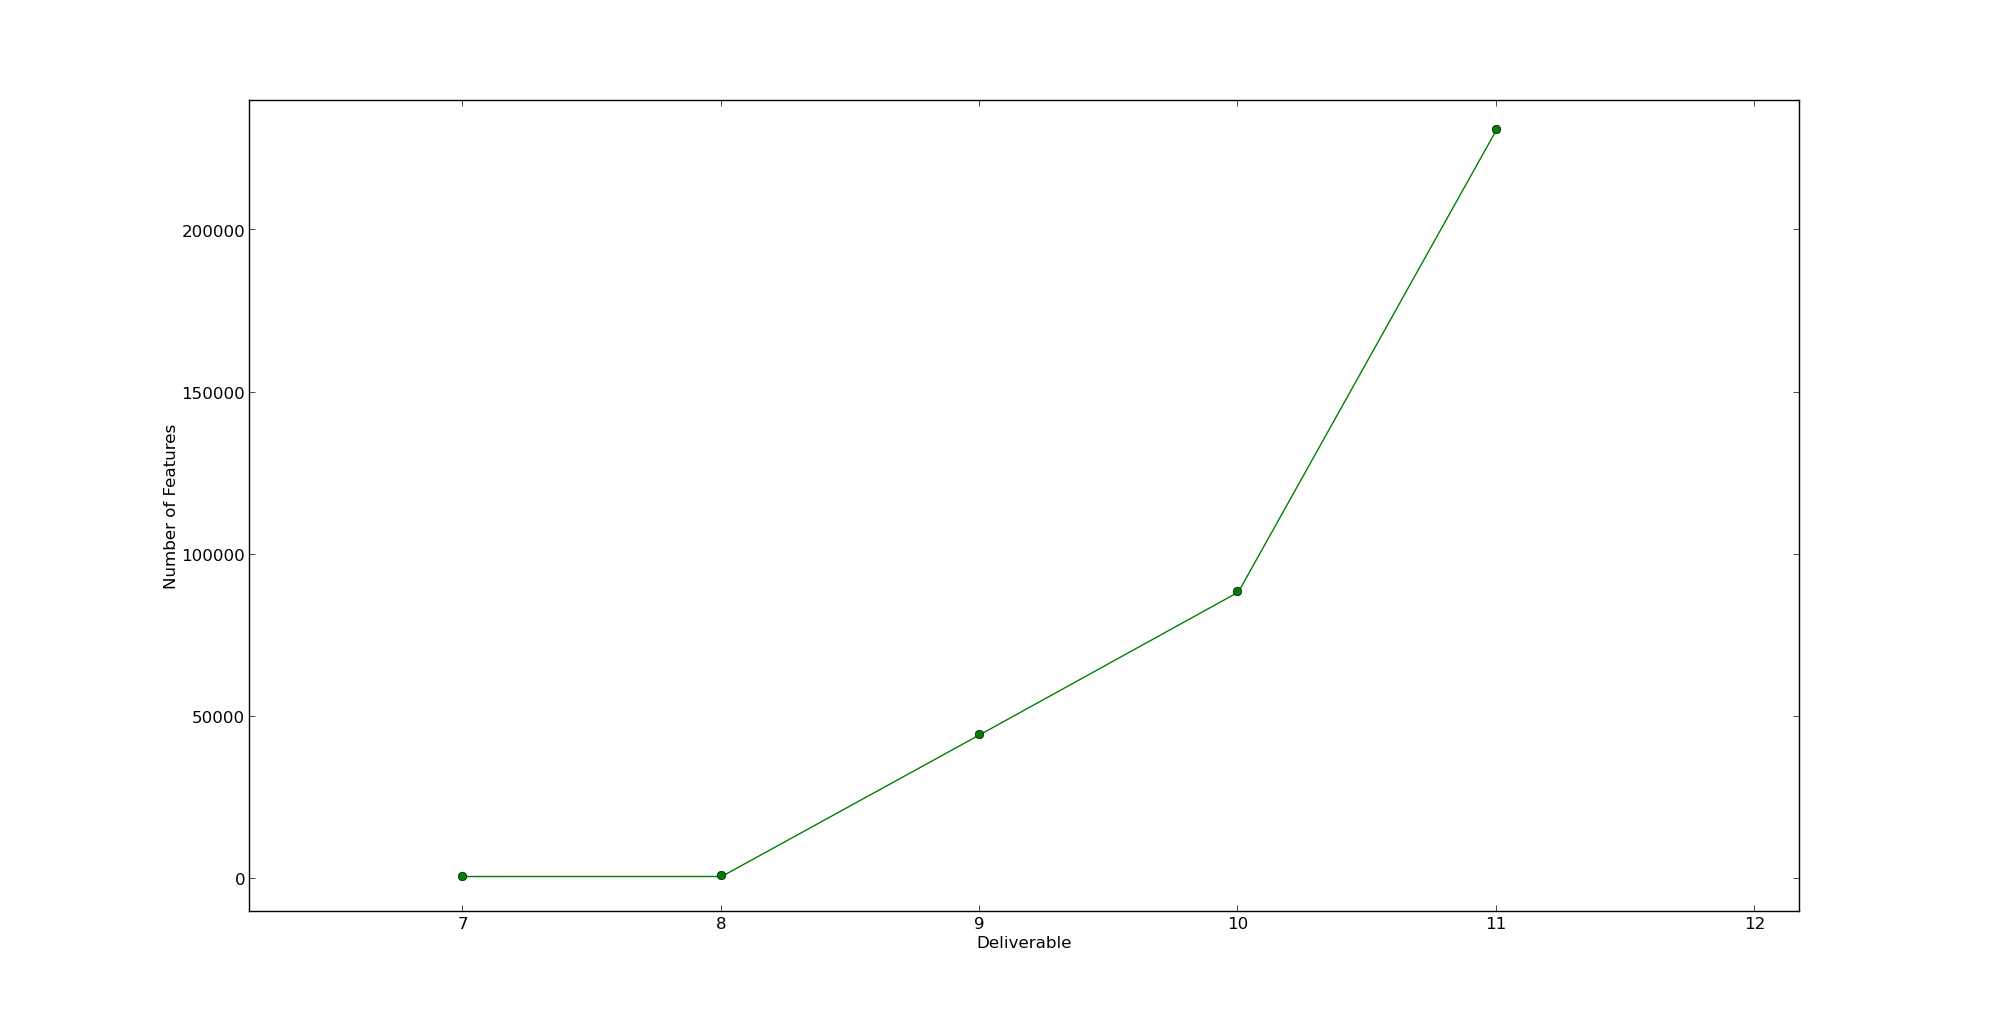
\includegraphics[scale = 0.25]{Images/fig}
    \caption{Increase in Feature Count (first two data points correspond to 801 and 814 respectively)}
  \label{fig}
\end{figure}


\subsection{Bakeoff}
\subsubsection*{Deliverable 12}
My best feature set consists of all the tag combinations that I have used from deliverable 8 to deliverable 11. After running the \textbf{dp.test()} function, I get the file \textit{``english test.conll.pred''}. I have renamed it as \textit{``jagannathan.conll.pred''} which is my submission for the bake off.


\section{7650: Applications of Dependency Parsing}
\subsubsection*{Deliverable 13}
The paper I have chosen for Literature Review is `\textbf{`Quadratic-time dependency parsing for machine translation''} \cite{galley2009quadratic} which utilizes dependency parsing to perform a phrase-based decoding/translation from Chinese to English and vice-versa.

\subsubsection*{Problem Addressed}
The primary problem which the authors focus on is an \textbf{efficient} machine translation model, with respect to both speed (which is their top priority) and accuracy, of translating text in English to Chinese and vice-versa. The authors describe a technique to utilize maximum spanning tree (MST) parsing to machine translation, and how it can be integrated into a phrase-based decoder to compute dependency language model scores for a pair of source and target language.
\subsubsection*{Rationale behind using dependency parsing}
There are two approaches that could be employed for machine translation - hierarchical and phrase-based. Hierarchical approaches \cite{chiang2005hierarchical}, construct a tree-structure for each sentence, consisting of phrases which are recursively constructed using sub-phrases. A context free grammar could be constructed for such a hierarchical model, and sentences could be parsed using the CKY algorithm, and a translation could be performed for each parse. When this approach is applied, using a m-gram language model, the time complexity would be $\bigO(n^{3m})$ where $n$ is the length of the sentence.

However the authors point out the results of the 2008 Open MT evaluation reveal that although many of the best systems performing Chinese-English translation incorporate such CFG models, they only perform slightly better than the best phrase-based parsers which utilize dependency parsing. The authors build on the dependency parsing algorithm of McDonald et al \cite{mcdonald2005non} which has a time complexity of $\bigO(n^2)$ rather than ``full-fledged'' chart parsing techniques, which take $\bigO(n^3)$ time, because (a) the difference in parsing accuracy is lower than 1\% and (b) The authors favor a parser which has a lower time complexity since the translation process does not require state-of-the-art parsing techniques to be employed.

Thus, the authors use an \textit{unlabeled} and non-projective dependency parsing technique. The parse tree is non-projective - meaning it may have crossing edges and the dependencies between the head and the modifier are not required to be nested. This relaxation is what allows the time complexity to be $\bigO(n^2)$. An interesting point mentioned in the paper is that, the time complexity still remains to be quadratic even if the order of the language model increases.
\subsubsection*{Methodology}
\begin{itemize}
	\item The dependency parsing is viewed as a simple sequence labeling task in which each word will be labeled with a ``head''. A pseudo ``root'' is assigned which will be the only word not to have a head.
	\item Their dependency parser uses a standard linear model to score each dependency relation. This is of the form,\\
	$s(i,j) = \lambda.\textbf{f}(i,j)$
	\item $\lambda$ corresponds to a weight vector which is obtained after training a structured perceptron augmented by MIRA.
	\item The score of the full tree is computed as a score of all the edges, \\
	$s(x,y) = \sum_{(i,j)\in \textbf{y}} \lambda. \textbf{f}(i,j)$
	\item Since this forms a directed graph, the Chu-Liu-Edmonds (CLE) algorithm is applied to find a maximum spanning tree out of it.
	\item During the application of CLE algorithm, while choosing the highest scoring edge for each modifier, the following translation information is generated by the translation decoder for the expansion,
		\begin{enumerate}
			\item A partial translation \textbf{x}
			\item A coverage set for the input words \textbf{c}
			\item A translation score $\sigma$
			\item A predicted POS tag $t_j$
			\item A dependency score $s_j$
		\end{enumerate}
	\item A modification which the authors make to the CLE algorithm is that they do not identify loops every time there is an expansion of nodes. Instead they just reflect that in the dependency score.
\end{itemize}

\subsubsection*{Features used}
The authors use features for the dependency parsing as well as for the phrase-based decoder. The features used for dependency parsing are,
\begin{enumerate}
	\item \textbf{Unigram features}: h-word, h-pos, h-word \& h-pos, m-word, m-pos, m-word \& m-pos, where ``h-'' and ``m-'' correspond to the head word and modifier word respectively.
	\item \textbf{Bigram features}: h-word \& m-word, h-pos \& m-pos, h-word \& h-pos \& m-word, h-word \& h-pos \& m-pos, m-word \& m-pos \& h-word, m-word \& m-pos \& h-pos, h-word \& h-pos \& m-word \& m-pos
	\item \textbf{Adjacent POS features}: h-pos \& h-pos+1 \& m-pos-1 \& m-pos, h-pos \& h-pos+1 \& m-pos \& m-pos+1, h-pos-1 \& h-pos \& m-pos-1 \& m-pos, h-pos-1 \& h-pos \& m-pos \& m-pos+1
	\item \textbf{In-between features}: h-pos \& h-pos + k \& m-pos , where k$\in$ [i, min(i+5, j)] \\
	h-pos \& m-pos - k \& m-pos, where k$\in$ [max(i, j-5), j] (5 is the upper bound and -5 is the lower bound for the distance between head and the modifier as considered by the authors).
\end{enumerate}
Here h-pos, m-pos refer to the POS tag of the head and modifier and h-word and m-word refer to the head word and modifier word. An offset of +k or -k indicate k elements to the right or left respectively.

The features used to perform decoding are,
\begin{enumerate}
	\item Phrase-based translational probabilities
	\item Lexically-weighted probabilities
	\item Word penalties, phrase penalties and linear distortions
	\item Language model score
\end{enumerate}

\subsubsection*{Results}
In this paper, the authors present the results of experiments run on Chinese-to-English language pairs. The training data consists of
about 28 million English words and 23.3 million Chinese words drawn from various news parallel corpora distributed by the Linguistic Data Consortium (LDC).

Chinese words were segmented with a conditional random field classifier \cite{chang2008optimizing}. The authors built a large 5-gram language model for both English and Chinese, and performed Kneser-Ney smoothing (removing 4-grams and 5-grams occurring less than 3 times in training data). The authors used the NIST MT evaluation data for Chinese from 2002 to 2008 for performing the training and testing. Each Chinese sentence in this corpus has four corresponding English reference sentences. The authors present their results based on evaluation of their experiments on two metrics (a) BLEU and (b) TER
\begin{enumerate}
\item \textbf{BLEU}: Across all the data sets the authors were able to get a BLEU score of 32.29\% on average without using a dependency language model and 32.74\% after using a dependency language model.
\item \textbf{TER}: Across all the data sets the authors got a TER score of 58.02\% on average without using a dependency language model and 57.10\% on average after using a dependency language model.
\end{enumerate}

The authors also present the results on the data broken down by genre. These are presented in Table \ref{broken}
\begin{table}[htbp]
\centering
\begin{tabular}{|r|l|l|l|l|}
\hline
\multicolumn{ 5}{|c|}{\textbf{BLEU [\%]}} \\ \hline
\multicolumn{1}{|l|}{Dependency Language Model} & newswire & web & speech & all \\ \hline
no & \multicolumn{1}{r|}{32.86} & \multicolumn{1}{r|}{21.75} & \multicolumn{1}{r|}{36.88} & \multicolumn{1}{r|}{32.29} \\ \hline
yes & \multicolumn{1}{r|}{33.19} & \multicolumn{1}{r|}{22.64} & \multicolumn{1}{r|}{37.51} & \multicolumn{1}{r|}{32.74} \\ \hline
\multicolumn{1}{|l|}{} &  &  &  &  \\ \hline
\multicolumn{ 5}{|c|}{\textbf{TRE [\%]}} \\ \hline
\multicolumn{1}{|l|}{Dependency Language Model} & newswire & web & speech & all \\ \hline
no & \multicolumn{1}{r|}{57.73} & \multicolumn{1}{r|}{62.64} & \multicolumn{1}{r|}{55.16} & \multicolumn{1}{r|}{58.02} \\ \hline
yes & \multicolumn{1}{r|}{56.73} & \multicolumn{1}{r|}{61.97} & \multicolumn{1}{r|}{54.26} & \multicolumn{1}{r|}{57.1} \\ \hline
\end{tabular}
\caption{Results of Machine Translation Broken Down by Genre}
\label{broken}
\end{table}

With respect to timing measures, in the case of English translations of 40 words and shorter, the baseline system took 6.5 seconds
per sentence, whereas the dependency LM system spent 15.6 seconds per sentence, i.e., 2.4 times the baseline running time. In the case of translations longer than 40 words, average speeds were respectively 17.5 and 59.5 seconds per sentence, i.e., the dependency was only 3.4 times slower.

\subsubsection*{Differences from (and Improvements to) existing methods}

The non-projective dependency parser presented by the authors improves upon the cubic time implementations already in existence, with very little loss of accuracy. Also their translation results provide a 0.92\% TER and 0.45\% BLEU absolute improvements. The authors claim that at the scale of data that their algorithm operates on, even such minor improvements are considerable achievements.


\bibliographystyle{unsrt}
\bibliography{myrefs}
\end{document}
%Helllo \cite{gimpel2010part} \cite{galley2009quadratic} \cite{klein2003accurate}